\documentclass{article}

%----------------------------------------
% Packages
%----------------------------------------
\usepackage[left=1in, right=1in, top=1in, bottom=1in]{geometry}
\usepackage{graphicx}
\usepackage{amsmath,amsbsy,amssymb,amsfonts,amsthm}
\usepackage{nicefrac}
\usepackage{mathtools}
\usepackage{color}
\usepackage{xspace} % Correct macro spacing
\usepackage[numbers]{natbib} % For citations
\usepackage{times}
\usepackage{graphicx,subfigure}
%\usepackage[small,bf]{caption}
\usepackage{algorithm,algorithmic} 
\usepackage{hyperref}
\usepackage{url}
\usepackage{booktabs}

\usepackage{xcolor}
\usepackage{shadethm}

\usepackage{import}
\import{../utils/}{macros.tex}

\usepackage{fancyhdr}
\pagestyle{fancy}
\lhead{This is my name}
\rhead{this is page \thepage}

\usepackage{fancyhdr}
\pagestyle{fancy}
\lhead{IFT 6085 - Theoretical principles for deep learning}
\rhead{Lecture 4: January 16, 2020}


\newshadetheorem{thm}{Theorem}
\newshadetheorem{defn}[thm]{Definition}
\newshadetheorem{assm}[thm]{Assumption}
\newshadetheorem{prop}[thm]{Property}
\newshadetheorem{eg}[thm]{Example}
\newshadetheorem{lemma}[thm]{Lemma}


\definecolor{shadethmcolor}{HTML}{F0F0F0}
%\definecolor{shadethmcolor}{HTML}{EDEDED}
%\definecolor{shadethmcolor}{HTML}{EDF8FF}
%\definecolor{shaderulecolor}{HTML}{EDF8FF}
%\definecolor{shaderulecolor}{HTML}{45CFFF}
\setlength{\shadeboxrule}{.4pt}


\setlength\parindent{0pt}

% Packages hyperref and algorithmic misbehave sometimes.  We can fix
% this with the following command.
\newcommand{\theHalgorithm}{\arabic{algorithm}}

%----------------------------------------
% Standard macros
%----------------------------------------


%----------------------------------------
% Project-specific macros
%----------------------------------------

%----------------------------------------
% Header
%----------------------------------------
\title{IFT 6085 - Lecture 4 \\ 
Black-Box Models and Lower bounds }
\date{}

%----------------------------------------
% Document
%----------------------------------------
\begin{document} 

%----------------------------------------
% Abstract
%----------------------------------------
\maketitle

\vspace{-0.5in}
\begin{center}
Please report any bugs to the scribes or instructor.
\end{center}
\vspace{0.2in}

\textbf{Scribes:}
\hfill
\textbf{Instructor:} Ioannis Mitliagkas

\textbf{Winter 2020:} Etienne Thuillier

\textbf{Winter 2019:} Ian Porada, Th\'eo Moins, William Starnaud 

\textbf{Winter 2018:} Sai Krishna, Krishna Murthy 


%----------------------------------------
% Body
%----------------------------------------

\newcommand{\infgc}{\inf_{g \in \mathcal{C}}}
\newcommand{\supgc}{\sup_{g \in \mathcal{C}}}

\newcommand{\Prob}{\mathbb{P}}
\newcommand{\E}{\mathbb{E}}
\newcommand{\reals}{\mathbb{R}}


\section{Summary}

In the previous lectures, we derived upper bounds on the convergence rate of \emph{gradient descent} for minimizing different classes of objective functions.
Specifically, we found that depending on the properties we have for the objective function (Lipschitz-continuity, convexity, strong convexity, and smoothness), we can obtain different upper bounds on the convergence rate of gradient descent minimizing this objective function. 
We also saw that these different bounds had different peculiarities; for instance, in some of the cases, it is the final iterate that appears in the bound and in the other cases, it is some weighted average of all the iterates. \\

In this lecture, we will summarize these previously derived upper bounds and observe their properties.
We will then derive a lower bound for the convergence rate of a black box model, which includes gradient descent, for minimizing a smooth, strongly convex objective function. 
Our definition of black box model encompasses a class of algorithms which includes \emph{gradient descent}.
Now, an upper bound on convergence rate is useful to see the efficiency of an algorithm, which is how many steps are needed to guarantee a result with a given precision. 
In contrast, a lower bound helps us aim for the best possible upper bound we could possibly obtain for a class of algorithms. 
Thus, we are able to restrict ourselves in future research for a better rate of convergence; if we found an approach that performs at the rate similar to the lower bound, it would be a waste of efforts to search for a better approach!
In this lecture, we will show that for a broad class of models, which includes gradient descent, there exists a (cleverly constructed) scenario for which we can prove a certain lower bound for its convergence rate.

\section{Convergence rate}

% \par The upper bounds on the convergence rate of gradient descent that we have derived in this class are summarized in Table~\ref{tab:upper_bounds}. In this table $D_1 = \|x_1-x^*\|_2$, where $x_1$ denotes the initial guess, and $x^*$ the closest optimal point.

% \begin{table}[H]
% \centering
% \renewcommand{\arraystretch}{1.8}
%  \begin{tabular}{|c | c |} 
%  \hline
%  \textbf{Properties of the Objective Function} & \textbf{Upper bound on Convergence Rate of Gradient Descent} \\
%  \hline
%  convex and L-Lipschitz & $\frac{D_1L}{\sqrt{T}}$   \\ 
%  \hline
%  convex and $\beta$-smooth &  $\frac{\beta D_1^2}{T}$\\
%  \hline
%  $\alpha$-strongly convex and L-Lipschitz & $\frac{L^2}{\alpha T}$ \\
%  \hline
%  $\alpha$-strongly convex and $\beta$-smooth & $\beta D_1^2 \exp(-\frac{4T}{\kappa})$ \\
%  \hline
% \end{tabular}
% \caption{Upper bounds on the convergence rate of gradient descent in relation to properties of the objective function.\label{tab:upper_bounds}}
% \end{table}
% \renewcommand{\arraystretch}{1}
\begin{table}[H]
\centering
    {
    \renewcommand{\arraystretch}{2.0}
    \begin{tabular}{cc}
    \toprule
		\textbf{Property of the Convex Objective Function} 
		& 
		\textbf{Upper Bound on Convergence Rate}
		\\
	\toprule
		$L-$Lipschitz & $ \frac{L D_1}{\sqrt{T}}$
	\\
% 	\midrule
		$\beta-$smooth & $ \frac{2 \beta D^2_1 }{T - 1}$
	\\
% 	\midrule
		$\alpha-$strongly convex and $L-$Lipschitz & $ \frac{2 L^2}{\alpha \left(T+1\right)}$
	\\
% 	\midrule
		$\alpha-$strongly convex and $\beta-$smooth & $ \frac{\beta D^2_1}{2} \exp({\frac{-4T}{\kappa + 1}})$
		\\
	\bottomrule
	\end{tabular}
	}
\caption{
    Upper bounds on the convergence rates for various function classes. Note that $D_1 := \left\lVert{\vx^{(1)} - \vx^*\right\rVert}_2$.
}
\label{tab:upper_bounds}
\end{table}
\renewcommand{\arraystretch}{1}

We can see that assuming smoothness leads to a faster convergence rate as compared to the case when the objective is assumed to only be $L$-Lipschitz.
When we assume additional properties, strong convexity and smoothness for instance, we get exponential convergence, which is our best upper bound so far. 
Some authors also refer to this as \emph{linear} convergence, due to the fact that a semi-logarithmic plot was usually used for convergence rates and an exponential convergence on such a plot yields a straight line.\\

Note that, under strongly convex and Lipschitz assumptions (i.e., the third row in Table~\ref{tab:upper_bounds}), the upper bound is independent of the distance between the optimal point and the initial iterate. 
This can seem counter-intuitive. 
However, note that a function cannot be both strongly convex and Lipschitz-continuous globally on an unbounded domain. 
Indeed, strong convexity implies that the gradient increases in an unbounded fashion with distance to the optimal; think of a parabola for visualization.
On the contrary, Lipschitz continuity requires that said gradient be bounded everywhere on the domain, however far from the optimal; think of a straight line for visualization. 
Hence, both conditions can hold together locally only within a region around the optimal point as shown in Fig.\ref{fig:l_lipschitz_alpha_conv}. 
Thus, the location of the initial guess is de facto restricted to this region, which leads to the lack of dependence on the initial guess.
However, both $\alpha$ (of $\alpha-$strong convexity) and $L$ (of $L-$Lipschitz continuity) appear in the upper bound because of the above discussion. 
Please refer to Theorem 3.9 from~\cite{bubeck} for more details.
% We do not provide a more detailed treatment of this question here. See theorem 3.9 from \cite{bubeck}.

\begin{figure}[h]
    \centering
    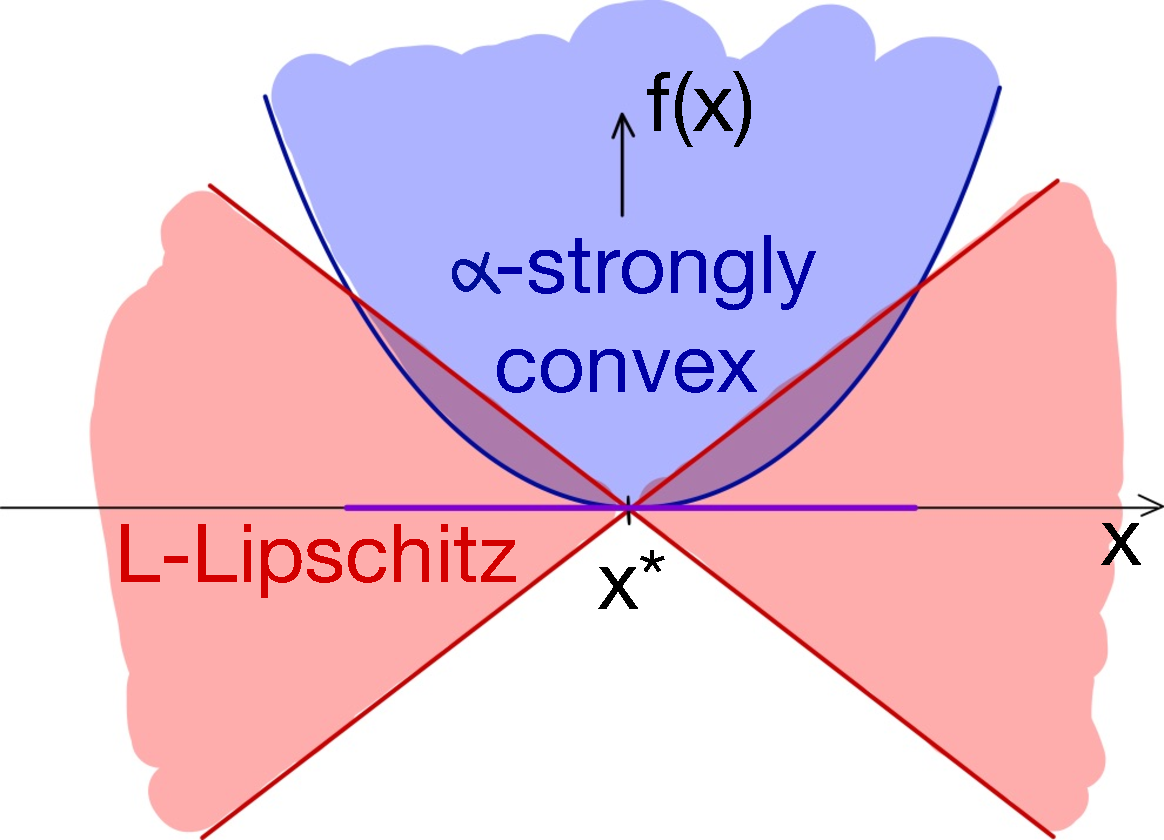
\includegraphics[scale=0.15]{img/L_Lipschitz_alpha_convex.pdf}
    \caption{The admissible domain (in purple) is compact under $L$-Lipschitz and $\alpha$-convex  conditions.\label{fig:l_lipschitz_alpha_conv}}
\end{figure}

\section{Black box models, the oracle, and taxonomy of different methods}
\label{blackbox}

A black box model assumes that the algorithm does not know the objective function $f$ being minimized.
However, the model does require information about the objective function in order to optimize it.
This information about the objective function can only be accessed by querying an \emph{oracle}. 
The oracle serves as a bridge between the unknown objective function and the optimizer; at any given step, the optimizer queries the oracle with a \emph{guess} $\vx$, and the oracle responds with information about the function at or around $x$.
This information may include the value of the function $f\left(\vx\right)$, the gradient of the function $\nabla f\left(\vx\right)$, the Hessian of the function $\nabla^2 f\left(\vx\right)$ and so on.
Intuitively, the oracle is used to represent what all type of information a black-box approach is allowed to use in order to optimize its objective, thereby allowing a categorization of the approaches as well as enabling analysis at a broader abstraction.
% (eg. value, gradient, Hessian, etc.). 
In particular, this framework proves to be suitable when we want to lower bound the asymptotic complexity of minimizing $f$ {\em regardless of what algorithm we use}. 
The complexity can be estimated as the number of queries that can be made to the oracle until we find an $\epsilon$-approximate minimum for the function $f$ at hand. 
Here we present a brief taxonomy of optimization methods, based on the nature of information about the function that the methods require.
 
\subsection{Zeroth order methods} 
These methods only require the value $f\left(\vx\right)$ of the function $f$ at the current guess $\vx$. 
They do not access any other \emph{higher-level} information like gradients or the Hessian. 
For example, the bisection method, genetic algorithms, simulated annealing, and Metropolis method are a few techniques that {\em can} fall under this category.

\subsection{First order methods} 
These methods can require the value $f\left(\vx\right)$ and the first derivative (gradient or Jacobian) $\nabla f\left(\vx\right)$ of the function $f$ at the current guess $x$. 
These methods are widely used for optimization in machine learning problems and include gradient descent (with or without averaging), Polyak's momentum~\cite{polyak}, and Nesterov's accelerated gradient methods~\cite{nesterov}.

\subsection{Second order methods} 
These methods can require the value $f\left(\vx\right)$, the first derivative (gradient or Jacobian) $\nabla f\left(\vx\right)$, and the second derivative (Hessian) $\nabla^2 f\left(\vx\right)$ of the function $f$ at the current guess $x$. 
% These methods can require the value of the function $f$, its first derivative (gradient or Jacobian) $\nabla f$, and its second derivative (Hessian) $\nabla^2 f$ at the current guess $x$. 
These methods use information about the local curvature, which is encoded in the Hessian. 
Intuitively, these methods morph the optimization surface so that gradients do not oscillate noisily but point straight towards the optimum.
Thus, they usually converge in a smaller number of iterations.
However, each iteration is computationally intensive, as it typically involves an inversion of the Hessian, which essentially renders them inapplicable to large-scale machine learning approaches. 
Another characteristic of these methods is the \emph{self-tuning} property; the step-size (learning rate) is determined implicitly from the curvature information and need not be tuned as a hyper-parameter. 
Newton's method is a very popular example of a second order method\footnote{
    Another class of techniques, sometimes referred to as \emph{Quasi-Newton methods}, is frequently used by the machine learning community. 
    As the name suggests, these techniques attempt to estimate/approximate second order information by using only the first order information. 
    BFGS and L-BFGS are popular Quasi-Newton methods.
}. 
Improving the efficiency of these second-order algorithms is an active area of research.

\subsection{Adaptive methods and conjugate gradients} 
The methods we mentioned until this point assume that all dimensions of a vector-valued variable (or sometimes all variables in the objective function) have a common set of hyper-parameters. 
\emph{Adaptive methods} relax this assumption and allow for every variable (or sometimes every dimension of a vector) to have its own set of hyper-parameters like the learning rate, momentum, etc. 
Some popular methods under this paradigm that are used in training deep neural networks are AdaGrad~\cite{adagrad} and Adam~\cite{adam}. \\

Conjugate gradient descent is a technique that we will not deal with in this course. 
However, to summarize, it attains the exact minimum for a quadratic, with no sub-optimality, in exactly $d$ iterations, where $d$ is the dimensionality of the quadratic function. 
Exploiting conjugate gradients in deep network training is still an active area of research.


\newcommand{\supff}{\sup_{f \in \mathcal{F}}}

\section{Lower bounds}

Up until now, we have looked only at upper bounds on convergence rates for different classes of objectives that are optimized using gradient descent. 
We will now derive a lower bound for the convergence rate by cleverly constructing a special case objective function that is smooth and strongly-convex.

\subsection{Why are lower bounds useful?}
Lower bounds are useful because they help us in deciding the best possible rate of convergence that we can achieve for the given category of optimizer.
Without lower bounds, an unnecessary amount of research energy might be spent on designing better optimizers, even if the intended convergence rate improvement would be impossible within this category of algorithm. 
A caveat here is that even if we prove that each procedure has a lower bounded rate of convergence, we don't know if a specific method reaches this bound.\\

Figure~\ref{conv} is a visualization of the bounds on convergence rates described thus far. 
One spoiler is that, as implied by comparing the slopes of the lines in the plot, the convergence rates of gradient descent that we derived as of now are slower as compared to the lower bound that we will derive! 
Thus, we are encouraged to search for better optimization methods that indeed attain the lower bound that we will see.
Another spoiler is that the convergence rate for the accelerated methods matches the lower bound that we will derive in all but a constant. 
% Again, note that any convergence rate below the lower bound is impossible for the black box models and objective functions under consideration.

\begin{figure}[h]
    \centering
    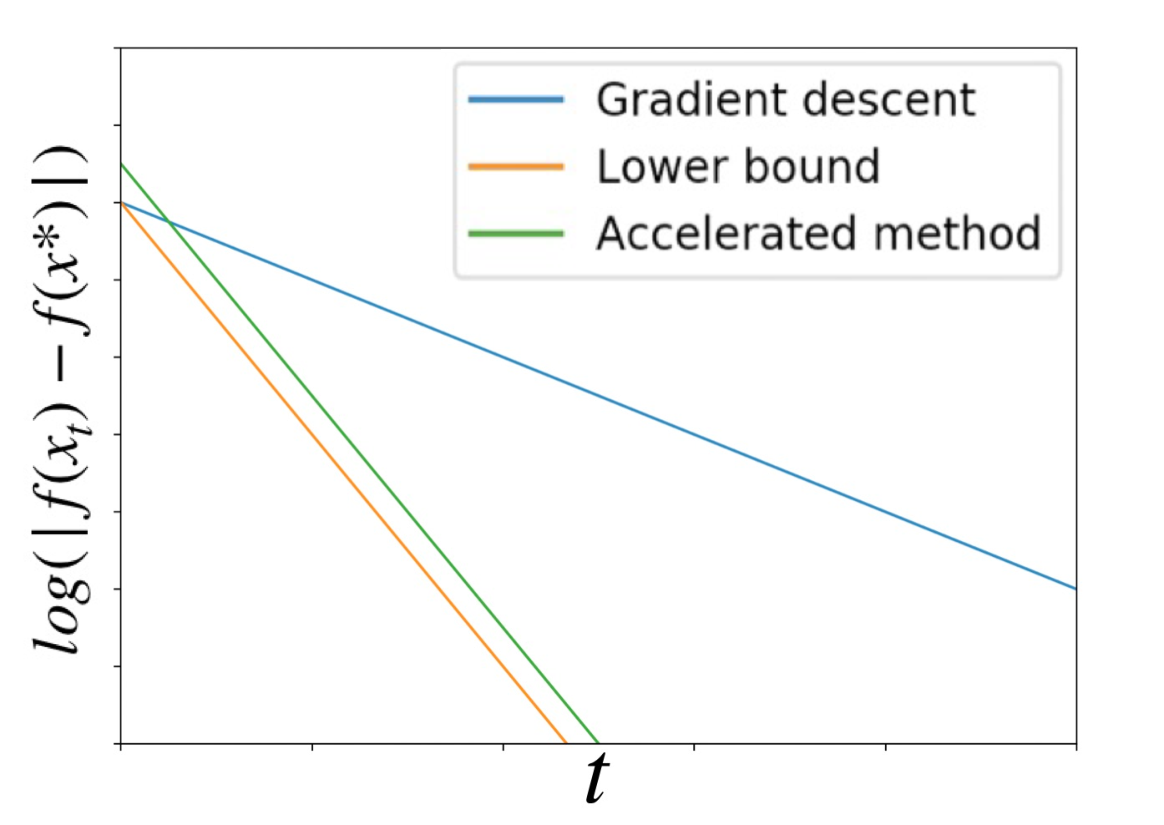
\includegraphics[scale=0.3]{img/gap.pdf}
    \caption{Converence rate for gradient descent and accelerated methods in comparison with lower bound}
    \label{conv}
\end{figure}


\subsection{Assumptions}
Under the black box model for first-order methods, we consider a sequence of iterates $\left\{\vx^{(t)}\right\}_{t = 1, 2, \ldots}$ and a sequence of gradients $\left\{\vg^{(t)}\right\}_{t = 1, 2, \ldots}$. 
The optimizer updates the variable $\vx$, which we interchangeably refer to as the parameter vector, using an update rule that satisfies the following criterion--
\begin{equation*}
    \forall\,t = 1, 2, \ldots,\ \text{we have}\ 
    \vx^{(t+1)} \in \text{span}\left(\vx^{(1)},     \vg^{(1)}, \vg^{(2)}, ..., \vg^{(t)} 
    \right)
\end{equation*}

This means that $\vx^{(t+1)}$ must be a linear combination of the initial iterate $\vx^{(1)}$ and the sequence of gradients $\left\{\vg^{(i)}\right\}_{i = 1}^t$ that are computed thus far in the algorithm. 
Note that $t$ is the index for the number of steps the optimizer is run for. 
Further, in our analysis, we assume that the initial guess $\vx^{(1)}$ is always the zero vector\footnote{
    It so happens that this assumption is indeed ``without any loss of generality''; the above model can easily be tweaked to hold for arbitrary initializations.
    However, in that case, the bounds that we obtain become tedious to work with, obfuscating the important stuff.
    Thus, the assumption is only for algebraic simplicity as we are primarily interested in the asymptotic rate.
}, i.e., $\vx^{(1)} = \mathbf{0}$.
% the above model can easily be tweaked to hold for arbitrary initializations, but in that case, expressions for bounds become tedious. We only make this assumption for algebraic simplicity, because we are interested in bounds on asymptotic rates. \footnote{If the initial guess was not the zero vector, but $x_{init}$, the update rule criterion must be modified to $x_{t+1} \in span\left( x_{init}, g_1, g_2, ..., g_t \right)$}


\subsection{Lower bounds for smooth and strongly convex objectives}
Now, we proceed to derive a lower bound for an objective function which is $\alpha$-strongly convex and $\beta$-smooth. 
However, before stating the result, we prove a set of important results that we would need.
\begin{thm}
(Gershgorin circle theorem) 
\label{thm:gersh}
Consider a complex matrix $\mA = \left[\emA_{i, j}\right]_{1\leq i, j\leq n}\in\mathbb{C}^{n\times n}$. 
For each row of the matrix, consider the sum of the absolute values/magnitudes of the non-diagonal entries of the row, i.e.,$\forall\,i\ \text{such that}\ 1\leq i\leq n$, let $R_i:=\sum\nolimits_{1\leq j\leq n, j\ne i} \left\lvert \emA_{i, j} \right\rvert$.
Let $i-$th Gershgorin disk $D_{i}\left(\emA_{i, i}, R_i\right)$ be defined as the disk in the complex plane with center $\emA_{i, i}$ and radius $R_i$.
Then, every eigenvalue $\lambda$ of $\mA$ lies within at least one of the $n$ Gershgorin disks.
\end{thm}
\begin{proof}
Let $\left(\lambda, \vv\right)$ be an eigenpair of the matrix $\mA$. 
By definition, every eigenvector $\vv$ is non-zero and hence, has at least one non-zero component $\evv_k$ for some $k\ \text{such that}\ 1\leq k\leq n$.
Now, let $i$ denote the index of the non-zero entry of $\vv$ that has the largest absolute value/magnitude, i.e., $\left\lvert v_j\right\rvert \geq \left\lvert v_i\right\rvert\ \forall\, j\ne i$.
Then, notice that $\vv^\prime = \frac{1}{ v_i}\vv$ is also an eigenvector corresponding to the same eigenvalue $\lambda$.
Further, $\evv_i^\prime = 1$ and $\left\lvert\evv_j^\prime\right\rvert \leq 1\ \forall\, j\ne i$.
With this, we have--
\begin{align*}
    & \mA\vv^\prime = \lambda\vv^\prime\ 
    \tag{eigenpair definition}
    \nonumber\\
    &
    \Longrightarrow
    \sum\nolimits_{j = 1}^n \emA_{i, j}\evv^\prime_j
    =
    \sum\nolimits_{1\leq j\leq n, j\ne i} \emA_{i, j}\evv^\prime_j
    +
    \emA_{i, i}
    =
    \lambda\evv^\prime_i
    =
    \lambda
    \ \ \ 
    \tag{$i-$th row of the matrix equation above and $\evv_i^\prime = 1$}
    \nonumber\\
    &
    \Longrightarrow
    \left\lvert
        \lambda - \emA_{i, i}
    \right\rvert
    =
    \left\lvert
        \sum\nolimits_{1\leq j\leq n, j\ne i} \emA_{i, j}\evv^\prime_j
    \right\rvert
    \leq 
    \sum\nolimits_{1\leq j\leq n, j\ne i}
    \left\lvert
        \emA_{i, j}\evv^\prime_j
    \right\rvert\ 
    \tag{triangle inequality}
    \nonumber\\
    &
    \Longrightarrow
    \left\lvert
        \lambda - \emA_{i, i}
    \right\rvert
    \leq 
    \sum\nolimits_{1\leq j\leq n, j\ne i}
    \left\lvert
        \emA_{i, j}\evv^\prime_j
    \right\rvert
    =
    \sum\nolimits_{1\leq j\leq n, j\ne i}
    \left\lvert
        \emA_{i, j}
    \right\rvert
    \left\lvert
        \evv^\prime_j
    \right\rvert
    \leq 
    \sum\nolimits_{1\leq j\leq n, j\ne i}
    \left\lvert
        \emA_{i, j}
    \right\rvert\ 
    \tag{we have $\left\lvert\evv_j^\prime\right\rvert \leq 1\ \forall\, j\ne i$ by construction}
\end{align*}
Finally, we get that 
$
    \left\lvert
        \lambda - \emA_{i, i}
    \right\rvert
    \leq 
    \sum\nolimits_{1\leq j\leq n, j\ne i}
    \left\lvert
        \emA_{i, j}
    \right\rvert
$
and thus, by definition, $\lambda\in D\left(\emA_{i, i}, R_i\right)$.
\end{proof}
\noindent Intuitively, Gershgorin circle theorem gives an extremely quick way to locate where the eigenvectors of a complex matrix lie.
Now, we are ready to demonstrate the desired lower bound.
% However, the bound on the location of the eigenvalue is fairly \emph{weak}.
%%%%%%%%%%%%%%%%%%%%%%%%%%%%%%%%%%%%%%%%
% Now, we prove a theorem that allows us to solve a special case of the so-called homogeneous systems of linear recurrence equations.
% That is quite a mouthful but the following theorem formalizes the simple underlying ideas.
% We will prove the result only for the \emph{case of degree 2}; for further reading, generalized results, and their proofs, please refer to any analysis of homogeneous linear recurrence relation.
% A good and concise reference is~\cite{recurrences}.

% \begin{thm}
% \label{linearRec}
% Consider a sequence of scalars $\left\{\evx^{(i)}\right\}_{i = 0}^\infty$ such that it satisfies the following \emph{homogeneous system of linear recurrences}: $\exists\,a, b, c\in\mathbb{R}\ \text{with}\ a\ne 0\ \text{such that}\ \forall\, n\in\mathbb{N}\cup \left\{0\right\}, a\evx^{(n+2)} + b\evx^{(n+1)} + c\evx^{(n)} = 0$.
% Consider the \emph{characteristic polynomial} of this system of equations, which is given by $P\left(x\right) = ax^2 + bx + c$. 
% Then, we have--
% \begin{align*}
%     &
%     \text{\textbf{1.}}\ 
%     \text{
%         If $P$ has two distinct roots $r_1, r_2$, then $\exists$ scalars $k_1, k_2$ such that $\evx^{(n)} = k_1 r_1^n
%         +
%         k_2 r_2^n
%         \, \forall,n\in\mathbb{N}\cup\left\{0\right\}$
%     }
%     \nonumber\\
%     &
%     \text{\textbf{2.}}\ 
%     \text{
%         If $P$ has repeated root $r$, then $\exists$ scalars $k_1, k_2$ such that $\evx^{(n)} = k_1 r^n
%         +
%         k_2 n r^n
%         \, \forall,n\in\mathbb{N}\cup\left\{0\right\}$
%     }
% \end{align*}
% \end{thm}
% \begin{proof}
% \textbf{1. }
% We prove the required result using strong induction.
% Suppose $P$ has two distinct real roots $r_1, r_2$.
% We first show the highly intuitive induction step.
% Suppose $\exists\,T\geq 1$ such that the following holds true: there exist scalars $k_1, k_2$ such that $\forall\,t=0, 1, \ldots, T$, we have $\evx^{(t)} = k_1 r_1^t + k_2 r_2^t$.
% Now, we have the following manipulations for $\evx^{(T + 1)}$:
% \begin{align*}
%     \evx^{(T + 1)}
%     &
%     =
%     -\frac{b}{a} {\evx^{(T)}}
%     -\frac{c}{a} {\evx^{(T - 1)}}\ 
%     \tag{from the recurrence relation and the fact $a\ne 0$}
%     \nonumber\\
%     &
%     =
%     -\frac{b}{a} \left(k_1 r_1^T + k_2 r_2^T\right)
%     -\frac{c}{a} \left(k_1 r_1^{T - 1} + k_2 r_2^{T-1}\right)\ 
%     \tag{induction hypothesis}
%     \nonumber\\
%     &
%     =
%     k_1 r_1^{T - 1}\left(
%         \frac{-b r_1 - c }{a}
%     \right)
%     +
%     k_2 r_2^{T - 1}\left(
%         \frac{-b r_2 - c }{a}
%     \right)
%     \nonumber\\
%     &
%     =
%     k_1 r_1^{T - 1}\left(
%         \frac{a r_1^2}{a}
%     \right)
%     +
%     k_2 r_2^{T - 1}\left(
%         \frac{a r_2^2}{a}
%     \right)\ 
%     \tag{$r_1, r_2$ are roots of $ax^2 + bx + c = 0$}
%     \nonumber\\
%     &
%     =
%     k_1 r_1^{T + 1}
%     +
%     k_2 r_2^{T + 1}
%     \Longrightarrow 
%     \evx^{(T + 1)}
%     =
%     k_1 r_1^{T + 1}
%     +
%     k_2 r_2^{T + 1}
% \end{align*}
% Thus, the only thing that remains is to establish the base cases for the induction to follow.
% In our case, we need to establish the base case for $T = 0$ and $T = 1$.
% In fact, this is the place where the special form of the root and the condition of two distinct roots comes into the picture.
% Specifically, consider the first two terms $\evx^{(0)}$ and $\evx^{(1)}$ of the given sequence of scalars and consider the following system of two equations in two unknowns $k_1, k_2$:
% \begin{align*}
% &
% \begin{array}{c}
%      k_1 r_1^0  + k_2 r_2^0 = \evx^{(0)}  
%      \\
%     k_1 r_1^1  + k_2 r_2^1 = \evx^{(1)} 
% \end{array}
% \Longrightarrow
% \begin{array}{c}
%     k_1\cdot 1 + k_2\cdot 1 = \evx^{(0)}  
%     \\
%     k_1\cdot r_1  + k_2\cdot r_2 = \evx^{(1)} 
% \end{array}
% \nonumber
% \end{align*}
% Since the two roots $r_1, r_2$ are distinct, we have the determinant 
% $
%     \left\lvert
%     \begin{array}{cc}
%         1 & 1 \\
%         r_1 & r_2 
%     \end{array}
%     \right\rvert
%     =
%     r_2 - r_1
%     \ne 0
% $.
% This gives that the system above has a unique solution for $\left(k_1, k_2\right)$.
% However, this system of equations in indeed obtained by setting the conditions for establishing the base case.
% Thus, $\exists$ a unique tuple of scalars $k_1, k_2$ such that $\evx^{(0)} = k_1 r_1^0 + k_2 r_2^0$ and $\evx^{(1)} = k_1 r_1^1 + k_2 r_2^1$.
% This base case with the above proof of the induction step completes the proof!\\[5pt]
% \textbf{2. }
% The proof for the case of repeated roots follows in an analogous manner; try it for yourself!
% \end{proof}
%%%%%%%%%%%%%%%%%%%%%%%%%%%%%%%%%%%%%%%%
% Now, we are ready to demonstrate the desired lower bound--
%The \emph{condition number} for a matrix will be denoted by $\kappa$. It is the ratio of the largest singluar value of the matrix to its smallest singluar value. If the condition number of a matrix is infinity, then the corresponding linear system is termed \emph{singular}. If the condition number is too large (but not infinity), then the corresponding linear system is termed \emph{ill-conditioned} (or \emph{poorly conditioned}). \\
\begin{thm}
\label{thethm}
(Theorem 3.15 from~\cite{bubeck})
There exists a $\beta$-smooth and $\alpha$-strongly convex function $f \colon \ell_2 \mapsto \mathbb{R}$ with condition number $\kappa = {\beta \over \alpha}$, with $\kappa > 1$, such that for any $t \geq 1$ and any \emph{black box procedure} with assumptions described in Section~\ref{blackbox}, the following lower bound holds.
\begin{equation}
    f(\vx^{(t)}) - f(\vx^\ast) \geq {\alpha \over 2}  \left( \frac{\sqrt[]{\kappa} - 1}{\sqrt[]{\kappa} + 1} \right)^{2(t-1)}  
    \left\lVert \vx^{(1)} - \vx^\ast\right\rVert^2
\end{equation} \\
Further, for large values of $\kappa$, we get the following asymptotic convergence rate--\\
\begin{equation}
 \left(\frac{\sqrt[]{\kappa} - 1}{\sqrt[]{\kappa} + 1} \right)^{2(t-1)} \approx \exp{ \left(-\frac{4(t-1)}{\sqrt[]{\kappa}}\right)}
\end{equation}
\end{thm}


\begin{proof}
We prove the lower bound by cleverly constructing an example function such that any black-box method with assumptions stated in Section~\ref{blackbox} gives the particular lower bound.
The example function we will construct is an $\ell_2$ function. 
Intuitively, $\ell_2$ functions are vectors with infinitely many coordinates that are square summable. 
Formally\footnote{To be even more formal, each element $\vx$ of $\ell_2$ is a real-valued sequence, and thus, a function from the set of natural numbers to reals.}, 
	\[
	    \ell_2 
	    := 
	    \left\{ 
	        \vx = \left(
	            \evx_1, \evx_2, \ldots
	   \right)\ \text{with}\ \evx_i\in\mathbb{R}\ \forall\,i\in\mathbb{N}\ 
	   \Big\lvert\ 
	       \sum_{i=1}^{\infty} x_i^2 < +\infty 
	    \right\}
	\]
    
Now, we define an operator $\mA$ that assumes the form of a tridiagonal matrix:
	\[ 
	   \mA 
	    = 
	    \left[ 
	        \begin{array}{cccccccc}
	            2 & -1 & 0 & \cdots & \cdots & \cdots & \cdots & \cdots \\ 
	            -1 & 2 & -1 & 0 & \cdots & \cdots & \cdots & \cdots \\ 
	            0 & -1 & 2 & -1 & 0 & \cdots & \cdots & \cdots \\ 
	            \vdots & 0 & -1 & 2 & -1 & 0 & \cdots & \cdots \\ 
	            \vdots & \vdots & 0 & -1 & 2 & -1 & 0 & \cdots \\ 
	            \vdots & \vdots & \vdots & \ddots & \ddots & \ddots & \ddots & \ddots  \end{array} 
	    \right] 
    \]
Now, we first want to establish where the eigenvalues of $\mA$ lie and for this, we use Gershgorin circle theorem from Theorem~\ref{thm:gersh}.
Notice that, by construction, $\mA$ has only two distinct Gershgorin disks, which are given by $D\left(2, 1\right)$ and $D\left(2, 2\right)$.
Further, notice that the former disk, which is centered at 1 and having a radius of 2, is entirely included in the latter disk, which is centered at 2 and has a radius of 2.
In addition, since $\mA$ is a symmetric operator, its eigenvalues are real.
Since Gershgorin circle theorem states that each eigenvalue must lie in at least one of the Gershgorin disks, combining all the previous observations gives that each eigenvalue lies in the Gershgorin disk $D\left(2, 2\right)$ and also on the real line.
Thus, each eigenvalue of $\mA$ must lie in the range $[0, 4]$.\\
% This operator has all its eigenvalues in the range [0,4].  This can be found by the use of Gershgorin disks\footnote{\url{https://en.wikipedia.org/wiki/Gershgorin_circle_theorem}}. First, we let $R_i = \sum_{j \neq i} |a_{ij}|$. Then we define the Gershgorin discs $D(a_{ii},R_i)$ of A as $D(a_{ii},R_{i}) = \left\{z\in {\mathbb  {C}},|a_{{ii}}-z|\leq R_i\right\}$. The Gershgorin circle theorem \cite{Ger31} then states that every eigenvalue of A must lie within at least one the discs $D(a_{ii},R_i)$.
% So with our expression of A, we only have two different discs, namely $D(2,1)$ and $D(2,2)$. The firs one is included in the latter one (i.e. $D(2,1) \subset D(2,2)$). Moreover, A is symmetrical, so the eigenvalues of A are real. We can infer that the eigenvalues of A must be in $[0,4]$.\\

Thus, we can define the following quadratic function $f:\ell_2\rightarrow \mathbb{R}$:
	\[
	    f(\vx) 
	    = 
	    \frac{\alpha \left(\kappa - 1\right)}{8}
	    \left(
	        \langle
	            \mA \vx, \vx
	        \rangle
	        -
	        2
	        \langle
	            \ve^{(1)}, \vx
	        \rangle
	    \right)
	    +
	    \frac{\alpha}{2}
	    \left\lVert\vx\right\rVert^2
	   % \left{
	   %     \alpha(\kappa-1) \over 8} \left( \langle Ax,x\rangle - 2\langle e_1,x \rangle \right) + {\alpha \over 2} \|x\|^2
	\]
Here, $\langle\cdot, \cdot\rangle$ denotes the vector inner-product and $\ve^{(1)}$ denotes the first vector of the canonical basis: $\ve^{(1)} := \left[ 
        1\quad 0\quad 0\quad \ldots
    \right]^\top$.
Now, we note a bunch of properties associated with this function.
First, since $\mA$ is symmetric, we have that
$$	
   \langle
	   \mA \vx, \vx
    \rangle 
    = 
    \left(\mA\vx\right)^\top \vx
    =
    \vx^\top A^\top\vx
    =
    \vx^\top A\vx
$$

Next, note that $f$ is $\alpha$-strongly convex by construction; the convex definition of the function along with the addendum ${\alpha \over 2} \|\vx\|^2$ term ensures that.
Also, $f$ is $\beta$-smooth; $\beta$-smoothness follows from the property that the eigenvalues of $\mA$ are bounded to be in the range $\left[0, 4 \right]$. 
Next, we compute the gradient of $f$:
\[
    \nabla f\left(\vx\right) 
    = 
    \frac{\alpha \left(\kappa - 1\right)}{4}
    \left(
        \mA\vx - \ve^{(1)}
    \right)
    +
    \alpha\vx
    % {\alpha (\kappa-1) \over 4} \left( Ax - e_1 \right) + \alpha x
\]    

As stated before, we will assume that the initial iterate is $\vx^{(1)} = \mathbf{0}$. 
Plugging this into the expression of gradient above, we get the gradient corresponding to $\vx = \vx^{(1)}$ as follows:
\[
    \vg^{(1)}
    =
    \left.\nabla f(\vx)\right{\Big\lvert}_{\vx = \vx^{(1)}} 
    = 
    -{\alpha (\kappa-1) \over 4} 
    \ve^{(1)} 
    = 
    \left[ 
        \begin{matrix}
	    -\alpha (\kappa-1) \over 4 
	    \\ 
	    0 
	    \\ 
	    0 
	    \\ 
	    \vdots
	    \end{matrix} 
	\right]
\]

Now, we utilize the fact that our black-box approach satisfies the assumption $
    \forall\,t = 1, 2, \ldots,\ \text{we have}\ 
    \vx^{(t+1)} \in \text{span}\left(\vx^{(1)},     \vg^{(1)}, \vg^{(2)}, ..., \vg^{(t)} 
    \right)$.
We have $\vx^{(1)} = \mathbf{0}$ and $\vg^{(1)}$ only has its component along $\ve^{(1)}$.
Thus, the next iterate 
$
    \vx^{(2)}
    \in
    \text{span}\left(
        \vx^{(1)}, \vg^{(1)}
    \right)
    =
    \text{span}\left( \ve^{(1)} \right)
$.
Thus, let $\vx^{(2)} = c_{2, 1}\ve^{(1)}$ for some scalar $c_{2, 1}\in\mathbb{R}$.
Now, we evaluate the gradient at $\vx^{(2)}$ as follows:
\[
    \vg^{(2)}
    =
    \left.\nabla f(\vx)\right{\Big\lvert}_{\vx = \vx^{(2)}} 
    = 
    -\frac{\alpha\left(\kappa - 1\right)}{4}
    \left(
        c_{2, 1}\mA\ve^{(1)}
        -
        \ve^{(1)}
    \right)
    \in 
    \text{span}\left(
        \ve^{(1)}, \ve^{(2)}
    \right)
\]
Here, the last step follows from observing that all the components of $\mA\ve^{(1)}$ after the first two are 0.
Thus, from the assumption 
$
    \vx^{(t+1)} 
    \in 
    \text{span}\left(\vx^{(1)},     \vg^{(1)}, \vg^{(2)}, ..., \vg^{(t)} \right)
$, we must have $\vx^{(3)}\in\text{span}\left(\vx^{(1)}, \vg^{(1)}, \vg^{(2)}\right) = \text{span}\left(\ve^{(1)}, \ve^{(2)}\right)$.
Thus, we have $\vx^{(3)} = c_{3, 1}\ve^{(1)} + c_{3, 2}\ve^{(2)}$ for some scalars $c_{3, 1}, c_{3, 2}\in\mathbb{R}$.\\

Continuing this way, we can prove using strong induction that for all iterates $\vx^{(t)}\ (t\in\mathbb{N})$, all the coordinates $\evx^{(t)}_i$ of $\vx^{(t)}$ with $i\geq t$ are 0, i.e., $\vx^{(t)}\in\text{span}\left(\ve^{(1)}, \ldots, \ve^{(t - 1)}\right)$.
This is a consequence of our design of the operator $\mA$.\\
% Using this expression, it is easy to show---by mathematical induction---that if $x_{t-1}$ has non-zero entries up to element at index $t-1$, then $x_{t}$ will have non-zero entries up to index $t$.
% The way the Hessian $A$ is designed, the non-zero values propagate across the dimensions, one dimension per each step of the gradient descent routine. That is, $x_t(i) = 0 \ \forall i \geq t$. Let's now consider the norm

Now, we know that $f$ has an optimal point, let us say at $\vx^\ast$, the existence of which is guaranteed by the strongly-convex nature of $f$.
With this, we consider the distance in the $t-$th iterate $\vx^{(t)}$ and the optimal point  $\vx^{\ast}$ as follows. 
\begin{align}
    \left\Vert
        \vx^{(t)} - \vx^\ast
    \right\rVert^2
	& 
	= 
	\sum\nolimits_{i=1}^{\infty} 
	\left( 
	    \evx^{(t)}_i - \evx^\ast_i
	\right)^2 
	=
	\sum\nolimits_{i=1}^{t - 1} 
	\left( 
	    \evx^{(t)}_i - \evx^\ast_i
	\right)^2 
	+
	\sum\nolimits_{i=t}^{\infty} 
	\left( 
	    \evx^{(t)}_i - \evx^\ast_i
	\right)^2 
	\nonumber\\
	 & 
	 \geq  
	 \sum\nolimits_{i=t}^{\infty} 
	\left( 
	    \evx^{(t)}_i - \evx^\ast_i
	\right)^2\ \tag{dropping a sum of squares, which is non-negative}
	\nonumber\\
	&
	=
	\sum\nolimits_{i=t}^{\infty} 
	\left( 
	    0 - \evx^\ast_i
	\right)^2
	=
	\sum\nolimits_{i=t}^{\infty} 
	\left(\evx^{\ast}_i\right)^2\ \tag{
	    $\evx^{(t)}_i = 0\ \forall\,i\geq t$
	}
\end{align}

Further, observe that we can relate the distance between the $t-$th iterate and the optimal point with the difference in the values taken by $f$ at these two points using strong-convexity of $f$.
Note that Lemma 6 of the previous lecture gives for an $\alpha-$strongly convex function, $f\left(\vx\right) - f\left(\vy\right)\geq \nabla f\left(\vy\right)^\top\left(\vx - \vy\right) + \frac{\alpha}{2}\left\lVert \vx - \vy \right\rVert^2\ \forall\,\vx,\vy$.
Setting $\vx\leftarrow\vx^{(t)}$ and $\vy\leftarrow\vx^{\ast}$, along with the fact that $\nabla f\left(\vx^{\ast}\right) = \mathbf{0}$, we get:
\begin{multline*}
    f(\vx^{(t)})
    -
    f(\vx^\ast)
    \geq 
    \nabla f\left(\vx^{\ast}\right)^\top
    \left(\vx^{(t)} - \vx^\ast\right)
    + 
    \frac{\alpha}{2}
    \left\lVert 
        \vx^{(t)} - \vx^{\ast}
    \right\rVert^2
    \\
    =
    \mathbf{0}^\top
    \left(\vx^{(t)} - \vx^\ast\right)
    + 
    \frac{\alpha}{2}
    \left\lVert 
        \vx^{(t)} - \vx^{\ast}
    \right\rVert^2
    =
    \frac{\alpha}{2}
    \left\lVert 
        \vx^{(t)} - \vx^{\ast}
    \right\rVert^2
\end{multline*}

Combining the previous two inequalities, we get:
$$
    \forall\,t,\ \text{we have}\ 
    f(\vx^{(t)})
    -
    f(\vx^\ast)
    \geq 
    \frac{\alpha}{2}
    \sum\nolimits_{i = t}^\infty
    \left(x^\ast_i\right)^2
$$

Here, we can intuitively see that we are on the right track.
This is because when we optimize $f$, the successive iterates $\vx^{(t)}$ are travelling closer and closer to $\vx^{\ast}$. 
And yet, we have shown that the separation between the values of $f$ at the $t-$th iterate $\vx^{(t)}$ and the optimal point $\vx^{\ast}$ has a lower bound, which we are interested in! 
The only thing that remains is to understand the rate of growth of the summation in the RHS of the inequality above, which we do next.\\
    
% Of course, as we keep running gradient descent, $\|x_t\|$ keeps getting smaller and smaller (if the learning rate is appropriately specified). Strong convexity gives us
% \begin{equation}
% 	\begin{split}
% 	f(x_t) - f(x^*) & \geq {\alpha \over 2} \| x_t - x^* \|^2 \\
% 	 & \geq {\alpha \over 2} \sum_{i=t}^{\infty} \left( x^*(i) \right)^2
% 	\end{split}
% \end{equation}

We know that $\vx^\ast$ is the optimal point of $\alpha-$strongly convex function $f$ and thus, we must have $\left.f\left(\vx\right)\right\Big\rvert_{\vx = \vx^\ast} = \mathbf{0}$.
Using the previously evaluated expression for $\nabla f$, we get the following:
\begin{align*}
    &\nabla f\left(\vx^\ast\right) 
    = 
    \frac{\alpha \left(\kappa - 1\right)}{4}
    \left(
        \mA\vx^\ast - \ve^{(1)}
    \right)
    +
    \alpha\vx^\ast
    =
    \mathbf{0}
    \Longrightarrow
        \frac{\left(\kappa - 1\right)}{4}\mA\vx
        +
        \vx
        =
        \frac{\left(\kappa - 1\right)}{4}\ve^{(1)}
\end{align*}
This is a vector equation, which gives an infinite family of equations where each equation corresponds to one dimension of the vector equation.
These equations are listed below.
\begin{align*}
    \left\{
        \begin{array}{ll}
            \frac{
                \left(\kappa - 1\right)
            }{4}
            \left(2\evx^{\ast}_1 - \evx^{\ast}_2 \right)
            +
            \evx^{\ast}_1
            =
            \frac{\left(
                \kappa - 1
            \right)}{4}
            &  {\left(\text{base case}\right)}
            \\
            \frac{\left(\kappa - 1\right)}{4}
            \left(
                -
                \evx^\ast_{t}
                +
                2\evx^\ast_{t + 1}
                -
                \evx^\ast_{t + 2}
            \right)
            +
            \evx^\ast_{t + 1}
            =
            0
            &
            \forall\,t\geq 1
        \end{array}
    \right.
    \Longrightarrow
    \left\{
        \begin{array}{ll}
            \evx^\ast_2
            -
            2
            \left(
                \frac{\kappa + 1}{\kappa - 1}
            \right)
            \evx^\ast_1
            +
            1
            =
            0
            & {\left(\text{base case}\right)}
            \\
            \evx^\ast_{t + 2}
            -
            2
            \left(
                \frac{\kappa + 1}{\kappa - 1}
            \right)
            \evx^\ast_{t + 1}
            +
            \evx^\ast_{t}
            =
            0
            &
            \forall\,t\geq 1
        \end{array}
    \right.
\end{align*}

Since $f$ is strongly convex, we just need to find a solution the above system of equations and the strong convexity would guarantee that it is the desired solution that we are looking for.
This system of equations (for $t\geq 1$) is the so-called \emph{linear homogeneous recurrence relations of degree 2} and it can be solved in a systematic manner.
Observe that setting $\vx^\ast$ with
$
    \evx^\ast_t 
    = 
    \left(
        \frac{\sqrt{\kappa} - 1}{\sqrt{\kappa} + 1}
    \right)^t\ \forall\,t\in\mathbb{N}
$ satisfies the above system\footnote{
    How did we cook up this solution?
    It so happens that this system of equations is a \emph{linear homogeneous recurrence relation system (of degree 2)}, which is a well-studied object.
    For interested readers, we show in Appendix~\ref{sec:appendix} a set of results related to solving such systems, which would reveal the motivation for this solution, and also demonstrate some of the nuances of the current proof.
    % We also refer the reader to a rigorous treatment of the generalized linear homogeneous recurrence relation systems of degree $d$.
} including the base case and for all $t\geq 1$.
Thus, as a consequence of the strong convexity of $f$, this is \emph{the} desired solution.
Now, we get the desired lower bound:
\begin{align*}
    \forall\,t,\ 
    f(\vx^{(t)})
    -
    f(\vx^\ast)
    &
    \geq 
    \frac{\alpha}{2}
    \sum\nolimits_{i = t}^\infty
    \left(x^\ast_i\right)^2
    \nonumber\\
    &
    =
    \frac{\alpha}{2}
    \sum\nolimits_{i = t}^\infty
    \left(
        \frac{
            \sqrt{\kappa} - 1
        }{
            \sqrt{\kappa} + 1
        }
    \right)^{2i}\ \tag{substituting the solution found above}
    \nonumber\\
    &
    =
    \frac{\alpha}{2}
    \sum\nolimits_{j = 1}^\infty
    \left(
        \frac{
            \sqrt{\kappa} - 1
        }{
            \sqrt{\kappa} + 1
        }
    \right)^{2\left(j + t - 1\right)}\ 
    \tag{change of variables: $i = j + t - 1$}
    \nonumber\\
    &
    =
    \frac{\alpha}{2}
    \left(
        \frac{
            \sqrt{\kappa} - 1
        }{
            \sqrt{\kappa} + 1
        }
    \right)^{2\left(t - 1\right)}
    \sum\nolimits_{j = 1}^\infty
    \left(
        \frac{
            \sqrt{\kappa} - 1
        }{
            \sqrt{\kappa} + 1
        }
    \right)^{2j}\ 
    \nonumber\\
    &
    =
    \frac{\alpha}{2}
    \left(
        \frac{
            \sqrt{\kappa} - 1
        }{
            \sqrt{\kappa} + 1
        }
    \right)^{2\left(t - 1\right)}
    \sum\nolimits_{j = 1}^\infty
    \left(
        \evx^\ast_i
    \right)^2\ 
    \tag{substituting back for the solution found above}
    \nonumber\\
    &
    =
    \frac{\alpha}{2}
    \left(
        \frac{
            \sqrt{\kappa} - 1
        }{
            \sqrt{\kappa} + 1
        }
    \right)^{2\left(t - 1\right)}
    \sum\nolimits_{j = 1}^\infty
    \left(
        0 - \evx^\ast_i
    \right)^2
    \nonumber\\
    &
    =
    \frac{\alpha}{2}
    \left(
        \frac{
            \sqrt{\kappa} - 1
        }{
            \sqrt{\kappa} + 1
        }
    \right)^{2\left(t - 1\right)}
    \left\lVert
        \vx^{(1)}
        -
        \vx^{\ast}
    \right\rVert^2\ 
    \tag{because $\vx^{(1)} = \mathbf{0}$ by construction}
\end{align*}
% If we differentiate $f$ and set $\nabla f$ to $0$, we obtain an infinite linear system, of the following form (using the definition of $A$):
% \begin{equation}\label{linsys}
%     \left\{
% 	\begin{aligned}
% 		& 1 - 2{\kappa + 1 \over \kappa - 1}x^*(1) + x^*(2) = 0, \\
%         & x^*(k-1) - 2{\kappa + 1 \over \kappa - 1}x^*(k) + x^*(k+1) = 0 \ \forall k \geq 2.
% 	\end{aligned}
% 	\right.
% \end{equation}
% The solution of the above system is given by
% \[
% x^*(i) = \left( \sqrt{\kappa}-1 \over \sqrt{\kappa}+1 \right)^i
% \]
% \emph{Hint for derivation:} We sum all rows in the linear system to obtain $1 - x^*(1) + \sum_{k=1}^\infty [2 - 2({\kappa+1 \over \kappa -1})]x^*(k)=0$. We put $x^*(k)=r^k \ \forall k \geq 1$ and we use the value of geometric series to solve for $r$. \\
% However, this is nothing but a set of \emph{linear homogeneous recurrence relations of degree 2} and thus, Theorem~\ref{linearRec} comes to the rescue!
% Notice that for the recurrences $\forall\,t\geq 1$ as stated above, the characteristic polynomial is $P(x) = x^2 -2\left(\frac{\kappa + 1}{\kappa - 1}\right)x + 1$. 
% Notice that the discriminant of $P$ is given by: $\Delta = \left(-2\left(\frac{\kappa + 1}{\kappa - 1}\right)\right)^2 - 4\cdot 1\cdot 1 = 4\left(\left(1+\frac{2}{\kappa - 1}\right)^2 - 1\right)$.
% Since $\kappa > 1$ is given, we get that $\Delta > 0$, which implies that $P$ has two distinct real roots $r_1, r_2$ as given below:
% \begin{align*}
%     r_{1,2}
%     =
%     \frac{
%         -\left(-2
%             \left(
%             \frac{
%                 \kappa + 1    
%             }{
%                 \kappa - 1
%             }
%             \right)
%         \right)
%         \pm
%         \sqrt{\Delta}
%     }{
%         2\cdot 1
%     }
%     =
%     \frac{\kappa + 1}{\kappa - 1}
%     \pm
%     \sqrt{
%         \frac{4}{\left(\kappa - 1\right)^2}
%         +
%         \frac{4}{\left(\kappa - 1\right)}
%     }
%     =
%     \frac{\kappa + 1 \pm 2\sqrt{\kappa}}{\kappa - 1}
%     =
%     \frac{
%         \left(\sqrt{\kappa}\pm 1\right)^2
%     }{
%         \left(\sqrt{\kappa} - 1\right)
%         \left(\sqrt{\kappa} + 1\right)
%     }
% \end{align*}
% Simplifying these expressions, we get the two roots as follows:
% \begin{align*}
%     r_1
%     =
%     \frac{
%         \sqrt{\kappa} + 1
%     }{
%         \sqrt{\kappa} - 1
%     }
%     \qquad\ \text{and}\ \qquad
%     r_2
%     =
%     \frac{
%         \sqrt{\kappa} - 1
%     }{
%         \sqrt{\kappa} + 1
%     }
% \end{align*}
% Now Theorem~\ref{linearRec} implies that there are scalars $c_1, c_2$ such that $\forall\,t\in\mathbb{N}$, we have:
% $
%     \evx^\ast_t 
%     = 
%     c_1 r_1^t
%     +
%     c_2 r_2^t
% $. 
% Plugging this into the base case above, we get:
% \begin{align*}
%     &
%     \evx^\ast_2
%             -
%             2
%             \left(
%                 \frac{\kappa + 1}{\kappa - 1}
%             \right)
%             \evx^\ast_1
%             +
%             1
%             =
%             0
%     \Longrightarrow
%     \left(c_1 r_1^2 + c_2 r_2^2\right)
%     -2
%     \left(
%         \frac{\kappa + 1}{\kappa - 1}
%     \right)
%     \left(
%         c_1 r_1 + c_2 r_2
%     \right)
%     +
%     1
%     = 
%     0
%     \nonumber\\
%     &
%     \Longrightarrow
%     c_1\left(
%         r_1^2 
%         -
%         2
%         \left(
%             \frac{\kappa + 1}{\kappa - 1}
%         \right)
%         r_1
%         + 
%         1
%     \right)
%     +
%      c_2\left(
%         r_2^2 
%         -
%         2
%         \left(
%         r_2
%             \frac{\kappa + 1}{\kappa - 1}
%         \right)
%         + 
%         1
%     \right)
%     +
%     1 - \left(c_1 + c_2\right)
%     = 
%     0
%     \nonumber\\
%     &
%     \Longrightarrow
%     c_1\cdot 0 + c_2\cdot 0
%     + 1 - \left(c_1 + c_2\right)
%     = 
%     0\ \tag{$r_1, r_2$ are roots of $P(x) = x^2 -2\left(\frac{\kappa + 1}{\kappa - 1}\right) + 1 $}
%     \Longrightarrow
%     c_2 = 1 - c_1
%     \nonumber
%     \\
%     &
%     \Longrightarrow
%     \forall\,t\in\mathbb{N},\ \evx^\ast_t = c_1\left(r_1^t - r_2^t\right) + r_2^t 
%     \nonumber
%     \\
%     &
%     \Longrightarrow
%     \forall\,t\in\mathbb{N},\
%     \left(\evx^\ast_t\right)^2 
%     = 
%     c_1^2 r_1^{2t}
%     +
%     \left(c_1^2 + 1\right) r_2^{2t}
%     -2c_1^2\ \tag{because $r_1\cdot r_2 = 1$}
%     +
%     2 c_1 
%     -
%     2 c_1 r_2^{2t}
% \end{align*}
% Now, we plug this into the above expression, which gives us
% \begin{equation}
% 	\begin{alignedat}{2}
% 	f(x_t) - f(x^*) & \geq {\alpha \over 2} \| x_t - x^* \|^2  &&\\
% 	 & \geq {\alpha \over 2} \sum_{i=t}^{\infty} (x_t^*(i))^2 &&\\
% 	  & = {\alpha \over 2} \sum_{i=t}^{\infty}  \left( \sqrt{\kappa}-1 \over \sqrt{\kappa}+1 \right)^{2i} && \text{(By solution to the linear system ($\ref{linsys}$) above)}\\
% 	  & = {\alpha \over 2} \sum_{i=1}^{\infty}  \left( \sqrt{\kappa}-1 \over \sqrt{\kappa}+1 \right)^{2(i+t-1)} &&\text{(By change of variable)}\\
% 	  &= \frac{\alpha}{2}\left({\sqrt{\kappa} - 1 \over \sqrt{\kappa} + 1}\right)^{2(t-1)} \sum_{i=1}^\infty \left({\sqrt{\kappa} - 1 \over \sqrt{\kappa} +1}\right)^{2i} &&\\
% 	  &= \frac{\alpha}{2} \left( \sqrt{\kappa} - 1 \over \sqrt{\kappa} + 1 \right)^{2(t-1)} \sum_{i=1}^{\infty} \left( x^*(i) \right)^{2} && \text{(By solution to the linear system ($\ref{linsys}$) above)}\\
% 	  & = {\alpha \over 2} \left( \sqrt{\kappa}-1 \over \sqrt{\kappa}+1 \right)^{2(t-1)}||x_1 - x^*||^2 && \text{(By derivation ($\ref{normsumeq}$) above for $x_1$)}
% 	\end{alignedat}
% \end{equation}
This completes the proof and provides us with the desired lower bound!

\end{proof}


\newcommand{\cf}{\mathbb{S}_{\mathcal{F}}}



%----------------------------------------
% \section*{Acknowledgments} 

%----------------------------------------
\bibliographystyle{abbrvnat}
\bibliography{Refs/lec4}

\newpage
%----------------------------------------
\section*{Appendix: Linear Homogeneous Recurrence Relations}
\label{sec:appendix}

\subsection*{Solving Recurrences}
Here, we prove a theorem that allows us to solve the so-called homogeneous systems of linear recurrence equations.
% That is quite a mouthful but the following theorem formalizes the simple underlying ideas.
We will prove the result only for the \emph{case of degree 2}; for further reading, generalized results, and their proofs, please refer to any analysis of linear homogeneous recurrence relations.
A good and concise reference for the same is~\cite{recurrences}.

\begin{thm}
\label{linearRec}
Consider a sequence of scalars $\left\{\evx^{(i)}\right\}_{i = 0}^\infty$ such that it satisfies the following \emph{homogeneous system of linear recurrences}: $\exists\,a, b, c\in\mathbb{R}\ \text{with}\ a\ne 0\ \text{such that}\ \forall\, n\in\mathbb{N}\cup \left\{0\right\}, a\evx^{(n+2)} + b\evx^{(n+1)} + c\evx^{(n)} = 0$.
Consider the \emph{characteristic polynomial} of this system of equations, which is given by $P\left(x\right) = ax^2 + bx + c$. 
Then, we have--
\begin{align*}
    &
    \text{\textbf{1.}}\ 
    \text{
        If $P$ has two distinct roots $r_1, r_2$, then $\exists$ scalars $k_1, k_2$ such that $\evx^{(n)} = k_1 r_1^n
        +
        k_2 r_2^n
        \, \forall,n\in\mathbb{N}\cup\left\{0\right\}$
    }
    \nonumber\\
    &
    \text{\textbf{2.}}\ 
    \text{
        If $P$ has repeated root $r$, then $\exists$ scalars $k_1, k_2$ such that $\evx^{(n)} = k_1 r^n
        +
        k_2 n r^n
        \, \forall,n\in\mathbb{N}\cup\left\{0\right\}$
    }
\end{align*}
\end{thm}
\begin{proof}
\textbf{1. }
We prove the required result using strong induction.
Suppose $P$ has two distinct real roots $r_1, r_2$.
We first show the highly intuitive induction step.
Suppose $\exists\,T\geq 1$ such that the following holds true: there exist scalars $k_1, k_2$ such that $\forall\,t=0, 1, \ldots, T$, we have $\evx^{(t)} = k_1 r_1^t + k_2 r_2^t$.
Now, we have the following manipulations for $\evx^{(T + 1)}$:
\begin{align*}
    \evx^{(T + 1)}
    &
    =
    -\frac{b}{a} {\evx^{(T)}}
    -\frac{c}{a} {\evx^{(T - 1)}}\ 
    \tag{from the recurrence relation and the fact $a\ne 0$}
    \nonumber\\
    &
    =
    -\frac{b}{a} \left(k_1 r_1^T + k_2 r_2^T\right)
    -\frac{c}{a} \left(k_1 r_1^{T - 1} + k_2 r_2^{T-1}\right)\ 
    \tag{induction hypothesis}
    \nonumber\\
    &
    =
    k_1 r_1^{T - 1}\left(
        \frac{-b r_1 - c }{a}
    \right)
    +
    k_2 r_2^{T - 1}\left(
        \frac{-b r_2 - c }{a}
    \right)
    \nonumber\\
    &
    =
    k_1 r_1^{T - 1}\left(
        \frac{a r_1^2}{a}
    \right)
    +
    k_2 r_2^{T - 1}\left(
        \frac{a r_2^2}{a}
    \right)\ 
    \tag{$r_1, r_2$ are roots of $ax^2 + bx + c = 0$}
    \nonumber\\
    &
    =
    k_1 r_1^{T + 1}
    +
    k_2 r_2^{T + 1}
    \Longrightarrow 
    \evx^{(T + 1)}
    =
    k_1 r_1^{T + 1}
    +
    k_2 r_2^{T + 1}
\end{align*}
Thus, the only thing that remains is to establish the base cases for the induction to follow.
In our case, we need to establish the base case for $T = 0$ and $T = 1$.
In fact, this is the place where the special form of the root and the condition of two distinct roots comes into the picture.
Specifically, consider the first two terms $\evx^{(0)}$ and $\evx^{(1)}$ of the given sequence of scalars and consider the following system of two equations in two unknowns $k_1, k_2$:
\begin{align*}
&
\begin{array}{c}
     k_1 r_1^0  + k_2 r_2^0 = \evx^{(0)}  
     \\
    k_1 r_1^1  + k_2 r_2^1 = \evx^{(1)} 
\end{array}
\Longrightarrow
\begin{array}{c}
    k_1\cdot 1 + k_2\cdot 1 = \evx^{(0)}  
    \\
    k_1\cdot r_1  + k_2\cdot r_2 = \evx^{(1)} 
\end{array}
\nonumber
\end{align*}
Since the two roots $r_1, r_2$ are distinct, we have the determinant 
$
    \left\lvert
    \begin{array}{cc}
        1 & 1 \\
        r_1 & r_2 
    \end{array}
    \right\rvert
    =
    r_2 - r_1
    \ne 0
$.
This gives that the system above has a unique solution for $\left(k_1, k_2\right)$.
However, this system of equations in indeed obtained by setting the conditions for establishing the base case.
Thus, $\exists$ a unique tuple of scalars $k_1, k_2$ such that $\evx^{(0)} = k_1 r_1^0 + k_2 r_2^0$ and $\evx^{(1)} = k_1 r_1^1 + k_2 r_2^1$.
This base case with the above proof of the induction step completes the proof!\\[5pt]
\textbf{2. }
The proof for the case of repeated roots follows in an analogous manner; try it for yourself!
\end{proof}

\begin{lemma}
Let $P(x) = ax^2 + bx + c\ \left(a, b, c\in\mathbb{R}\right)$.
Let $\lambda$ be a root of $P$.
Then, the sequence $\left\{x^{(n)}\right\}_{n = 1}^\infty$ defined by $x^{(n)} = \lambda^n$ satisfies the linear homogeneous recurrence relations $a\evx^{(n + 2)} + b\evx^{(n + 1)} + c\evx^{(n)} = 0\ \forall\,n\in\mathbb{N}$.
\end{lemma}
\begin{proof}
Trivial, try to prove for yourself!
\end{proof}

\subsection*{A Nuance in the Proof of Theorem~\ref{thethm}}
These results above reveal how we came up with the solution 
$
    \evx^{\ast}_t 
    = 
    \left(
        \frac{\sqrt{\kappa} - 1}{\sqrt{\kappa} + 1}
    \right)^t
$.
We solved for the characteristic polynomial of the involved recurrence: $P(x) = x^2 -2\left(\frac{\kappa + 1}{\kappa - 1}\right)x + 1$. 
% Notice that the discriminant of $P$ is given by: $\Delta = \left(-2\left(\frac{\kappa + 1}{\kappa - 1}\right)\right)^2 - 4\cdot 1\cdot 1 = 4\left(\left(1+\frac{2}{\kappa - 1}\right)^2 - 1\right)$.
% Since $\kappa > 1$ is given, we get that $\Delta > 0$, which implies that $P$ has two distinct real roots $r_1, r_2$ as given below:
% \begin{align*}
%     r_{1,2}
%     =
%     \frac{
%         -\left(-2
%             \left(
%             \frac{
%                 \kappa + 1    
%             }{
%                 \kappa - 1
%             }
%             \right)
%         \right)
%         \pm
%         \sqrt{\Delta}
%     }{
%         2\cdot 1
%     }
%     =
%     \frac{\kappa + 1}{\kappa - 1}
%     \pm
%     \sqrt{
%         \frac{4}{\left(\kappa - 1\right)^2}
%         +
%         \frac{4}{\left(\kappa - 1\right)}
%     }
%     =
%     \frac{\kappa + 1 \pm 2\sqrt{\kappa}}{\kappa - 1}
%     =
%     \frac{
%         \left(\sqrt{\kappa}\pm 1\right)^2
%     }{
%         \left(\sqrt{\kappa} - 1\right)
%         \left(\sqrt{\kappa} + 1\right)
%     }
% \end{align*}
It turns out that $P$ has two distinct real roots:
\begin{align*}
    r_1
    =
    \frac{
        \sqrt{\kappa} + 1
    }{
        \sqrt{\kappa} - 1
    }
    \qquad\ \text{and}\ \qquad
    r_2
    =
    \frac{
        \sqrt{\kappa} - 1
    }{
        \sqrt{\kappa} + 1
    }
\end{align*}
We chose $r_2$ and used the results above.
Note that in our solution, we did not have contributions from $r_1$ because $r_1 > 1$ and thus, leads to a lower bound that explodes.
Since our black box approach optimizes the objective so that $f(\vx^{(t)})$ approaches to $f(\vx^{\ast})$, thereby decreasing the gap, we will not have an exploding lower bound.
\end{document}
